\documentclass{article}
\usepackage[utf8]{inputenc}
\usepackage[margin=1in]{geometry}
\usepackage{amsmath}
\usepackage{amssymb}
\usepackage{pifont}
\newcommand{\xmark}{\ding{55}}%
\usepackage{fullpage}
\usepackage[english]{babel}
\usepackage{graphicx}
\usepackage{float}
\usepackage{hyperref}
\usepackage[usenames, dvipsnames]{color}
\usepackage{ragged2e}
\title{P2: Building an Intervention System}
\author{Naoki Shibuya}
\date{}

\begin{document}
\maketitle

\section{Classification vs Regression}

Your goal is to identify students who might need early intervention - which type of supervised machine learning problem is this, classification or regression? Why?\\
\color{blue}
This is a classification problem as the expected outcome has finite possibilities. In other words, they are discrete. In fact, it is a binary classification problem as the expected outcome is either 'yes' for students who require early intervention or 'no' for others who don't.
\color{black}

\section{Exploring the Data}

Can you find out the following facts about the dataset?

\begin{itemize}
\item Total number of students \textcolor{blue}{395}
\item Number of features (excluding the label/target column) \textcolor{blue}{30}
\item Number of students who passed \textcolor{blue}{265}
\item Number of students who failed \textcolor{blue}{130}
\item Graduation rate of the class (\%) \textcolor{blue}{67.09\%}
\end{itemize}

\section{Preparing the Data}

Execute the following steps to prepare the data for modeling, training and testing:

\begin{itemize}
\item Identify feature and target columns \\
\color{blue}
Feature column(s):-
['school', 'sex', 'age', 'address', 'famsize', 'Pstatus', 'Medu', 'Fedu', 'Mjob', 'Fjob', 'reason', 'guardian', 'traveltime', 'studytime', 'failures', 'schoolsup', 'famsup', 'paid', 'activities', 'nursery', 'higher', 'internet', 'romantic', 'famrel', 'freetime', 'goout', 'Dalc', 'Walc', 'health', 'absences'] \\
Target column: passed
\color{black}
\item Preprocess feature columns \\
\color{blue}
Processed feature columns (48):-
['school\_GP', 'school\_MS', 'sex\_F', 'sex\_M', 'age', 'address\_R', 'address\_U', 'famsize\_GT3', 'famsize\_LE3', 'Pstatus\_A', 'Pstatus\_T', 'Medu', 'Fedu', 'Mjob\_at\_home', 'Mjob\_health', 'Mjob\_other', 'Mjob\_services', 'Mjob\_teacher', 'Fjob\_at\_home', 'Fjob\_health', 'Fjob\_other', 'Fjob\_services', 'Fjob\_teacher', 'reason\_course', 'reason\_home', 'reason\_other', 'reason\_reputation', 'guardian\_father', 'guardian\_mother', 'guardian\_other', 'traveltime', 'studytime', 'failures', 'schoolsup', 'famsup', 'paid', 'activities', 'nursery', 'higher', 'internet', 'romantic', 'famrel', 'freetime', 'goout', 'Dalc', 'Walc', 'health', 'absences']
\end{itemize}
\color{black}

\section{Training and Evaluating Models}

Choose 3 supervised learning models that are available in scikit-learn, and appropriate for this problem. 
\\\\
For each model:
\begin{itemize}
\item What are the general applications of this model? What are its strengths and weaknesses?
\item Given what you know about the data so far, why did you choose this model to apply?
\item Fit this model to the training data, try to predict labels (for both training and test sets), and measure the F1 score. Repeat this process with different training set sizes (100, 200, 300), keeping test set constant.
\item Produce a table showing training time, prediction time, F1 score on training set and F1 score on test set, for each training set size.
\end{itemize}
Note: You need to produce 3 such tables - one for each model.
\\\\
\color{blue}
I'm using the following three learning models:
\\
\begin{itemize}
\item Decision Tree (sklearn.tree.DecisionTreeClassifier)
\\\\
\textbf{Pros} \\\\
Decision Tree is suitable for a classification problem with many features. It can actually handle categorical data so we would not need to convert categorical data into numerical data, which may reduce our time spent using the server time in production (if we choose to do so).\\
\\
It is a white box model in that a model's behaviour can be explained clearly since every decision inside a decision tree is a boolean logic. It'd be helpful when assessing and helping students who require early intervention.\\
\\
When predicting a target value, it requires the memory to look up the tree. It is reasonably fast in O(log2(n\_features)) time.
\\\\
\textbf{Cons} \\\\
The decision tree may become too large (more memory required) and hard to understand. It may overfit the data too easily with many features.
\\
\item Logistic Regression (sklearn.linear\_model.LogisticRegression)
\\\\
\textbf{Pros} \\\\
Logistic regression can map multiple explanatory variables into a binary value. Each feature gets a weight and as such it is helpful to assess students' situation.\\
\\
When predicting a target value, it has very low memory requirement, and very fast (constant time: O(1)).
\\\\
\textbf{Cons} \\
\\
While training, it may require lots of memory for large number of features if analytical solver is used. Otherwise, it may require more time as gradient descent needs to iteratively improve and approximate the best parameters.\\

\item SVM (sklearn.svm.SVC)
\\\\
\textbf{Pros} \\\\
SVM can handle multiple features and produce binary output.  It is less prone to overfitting (for example, comparing with Decision Tree).
\\\\
\textbf{Cons} \\
\\
SVM is a black box model.  It is like a line-drawing into a multi-dimensional space.  As such, it is not very clear how to understand the outcome when evaluating students who may require early intervention.\\
\end{itemize}
The following tables show the results of fitting each model to the training data and then predict labels for both training and test sets.
\begin{table}[H]
\centering
\begin{tabular}{| l | l | l | l |}
\hline
Traing set size           &  100 & 200 & 300 \\
\hline
Training time (secs)      & 0.001 & 0.001 & 0.002 \\
\hline
Prediction time (secs)    & 0.000 & 0.000 & 0.000 \\
\hline
F1 score for training set & 1.0  & 1.0  & 1.0  \\
\hline
F1 score for test set     & 0.765 & 0.679 & 0.713 \\
\hline
\end{tabular}
\caption{Decision Tree}
\end{table}

\begin{table}[H]
\centering
\begin{tabular}{| l | l | l | l |}
\hline
Traing set size           & 100 & 200 & 300 \\
\hline
Training time (secs)    & 0.001 & 0.002 & 0.002 \\
\hline
Prediction time (secs)  & 0.000 & 0.000 & 0.000 \\
\hline
F1 score for training set & 0.952 & 0.845 & 0.844 \\
\hline
F1 score for test set    & 0.761 & 0.710 & 0.759 \\
\hline
\end{tabular}
\caption{Logistic Regression}
\end{table}

\begin{table}[H]
\centering
\begin{tabular}{| l | l | l | l |}
\hline
Traing set size           & 100 & 200 & 300 \\
\hline
Training time (secs)      & 0.001 & 0.003 & 0.006 \\
\hline
Prediction time (secs)    & 0.001 & 0.002 & 0.004 \\
\hline
F1 score for training set & 0.923 & 0.854 & 0.883 \\
\hline
F1 score for test set     & 0.787 & 0.738 & 0.797 \\
\hline
\end{tabular}
\caption{SVM}
\end{table}

\color{black}

\section{Choosing the Best Model}

\begin{itemize}
\item Based on the experiments you performed earlier, in 2-3 paragraphs explain to the board of supervisors what single model you choose as the best model. 
\begin{itemize}
\item Which model has the best test F1 score and time efficiency? 
\item Which model is generally the most appropriate based on the available data, limited resources, cost, and performance? 
\end{itemize}
Please directly compare and contrast the numerical values recored to make your case.
\\
\color{blue}
\begin{itemize}
\item Training time (secs) 
\\\\
In terms of training time, Decision Tree is better than others.  As training size increases, SVM slows down much faster than the others.\\
\begin{table}[H]
\centering
\begin{tabular}{| l | l | l | l |}
\hline
Traing set size           & 100 & 200 & 300 \\
\hline
Decision Tree            & 0.001 & 0.001 & 0.002 \\
\hline
Logistic Regression      & 0.001 & 0.002 & 0.002 \\
\hline
SVM                      & 0.001 & 0.003 & 0.006 \\
\hline      
\end{tabular}
\caption{Logistic Regression Without Tuning}
\end{table}

\item Prediction time (secs)
\\\\
In terms of prediction time, Decision Tree and Logistic Regression takes almost no time.  SVM gets slower as more training data is used even though test set size remain constant, indicating SVM trained with more data requires more time and potentially more memory for prediction.
\\
\begin{table}[H]
\centering
\begin{tabular}{| l | l | l | l |}
\hline
Traing set size           & 100 & 200 & 300 \\
\hline
Decision Tree            & 0.000 & 0.000 & 0.000 \\
\hline
Logistic Regression      & 0.000 & 0.000 & 0.000 \\
\hline
SVM                      & 0.001 & 0.002 & 0.004 \\
\hline      
\end{tabular}
\caption{Logistic Regression Without Tuning}
\end{table}

\item F1 score for training set
\\\\
In terms of F1 score, both Logistic Regression and SVM performs well in all cases.  Decision Tree seems to overfit to the training data as it shows F1 score of 1 for training set and poor F1 score for test set (see the next section).  
\\
\begin{table}[H]
\centering
\begin{tabular}{| l | l | l | l |}
\hline
Traing set size           & 100 & 200 & 300 \\
\hline
Decision Tree             & 1.0  & 1.0   & 1.0  \\
\hline
Logistic Regression       & 0.952 & 0.845 & 0.844 \\
\hline
SVM                       & 0.923 & 0.854 & 0.883 \\
\hline      
\end{tabular}
\caption{Logistic Regression Without Tuning}
\end{table}

\item F1 score for test set
\\\\
In terms of training size, SVM performs best with smaller size.  However, Logistic Regression als performs as good if not better.  Decision Tree seems to require more than 300 training data to be able to make reasonable prediction which is unknown but we do not want such high requirement.  
\\
\begin{table}[H]
\centering
\begin{tabular}{| l | l | l | l |}
\hline
Traing set size           & 100  &  200  &  300 \\
\hline
Decision Tree            & 0.765 & 0.679 & 0.713 \\
\hline
Logistic Regression       & 0.761 & 0.710 & 0.759 \\
\hline
SVM                       & 0.787 & 0.738 & 0.797 \\
\hline      
\end{tabular}
\caption{Logistic Regression Without Tuning}
\end{table}

\item Other points about Decision Tree Classifier
\\\\
Decision Tree structure generated (see the graphviz output) is way too complicated to be used to assess student situation. I've tried grid search on max\_depth to see if reducing the complexity and avoiding overfitting proves to be better than other models. However, after the parameter tuning, Decision Tree still under-performs other models (see the below).
\\
\begin{table}[H]\centering
\begin{tabular}{c c}
       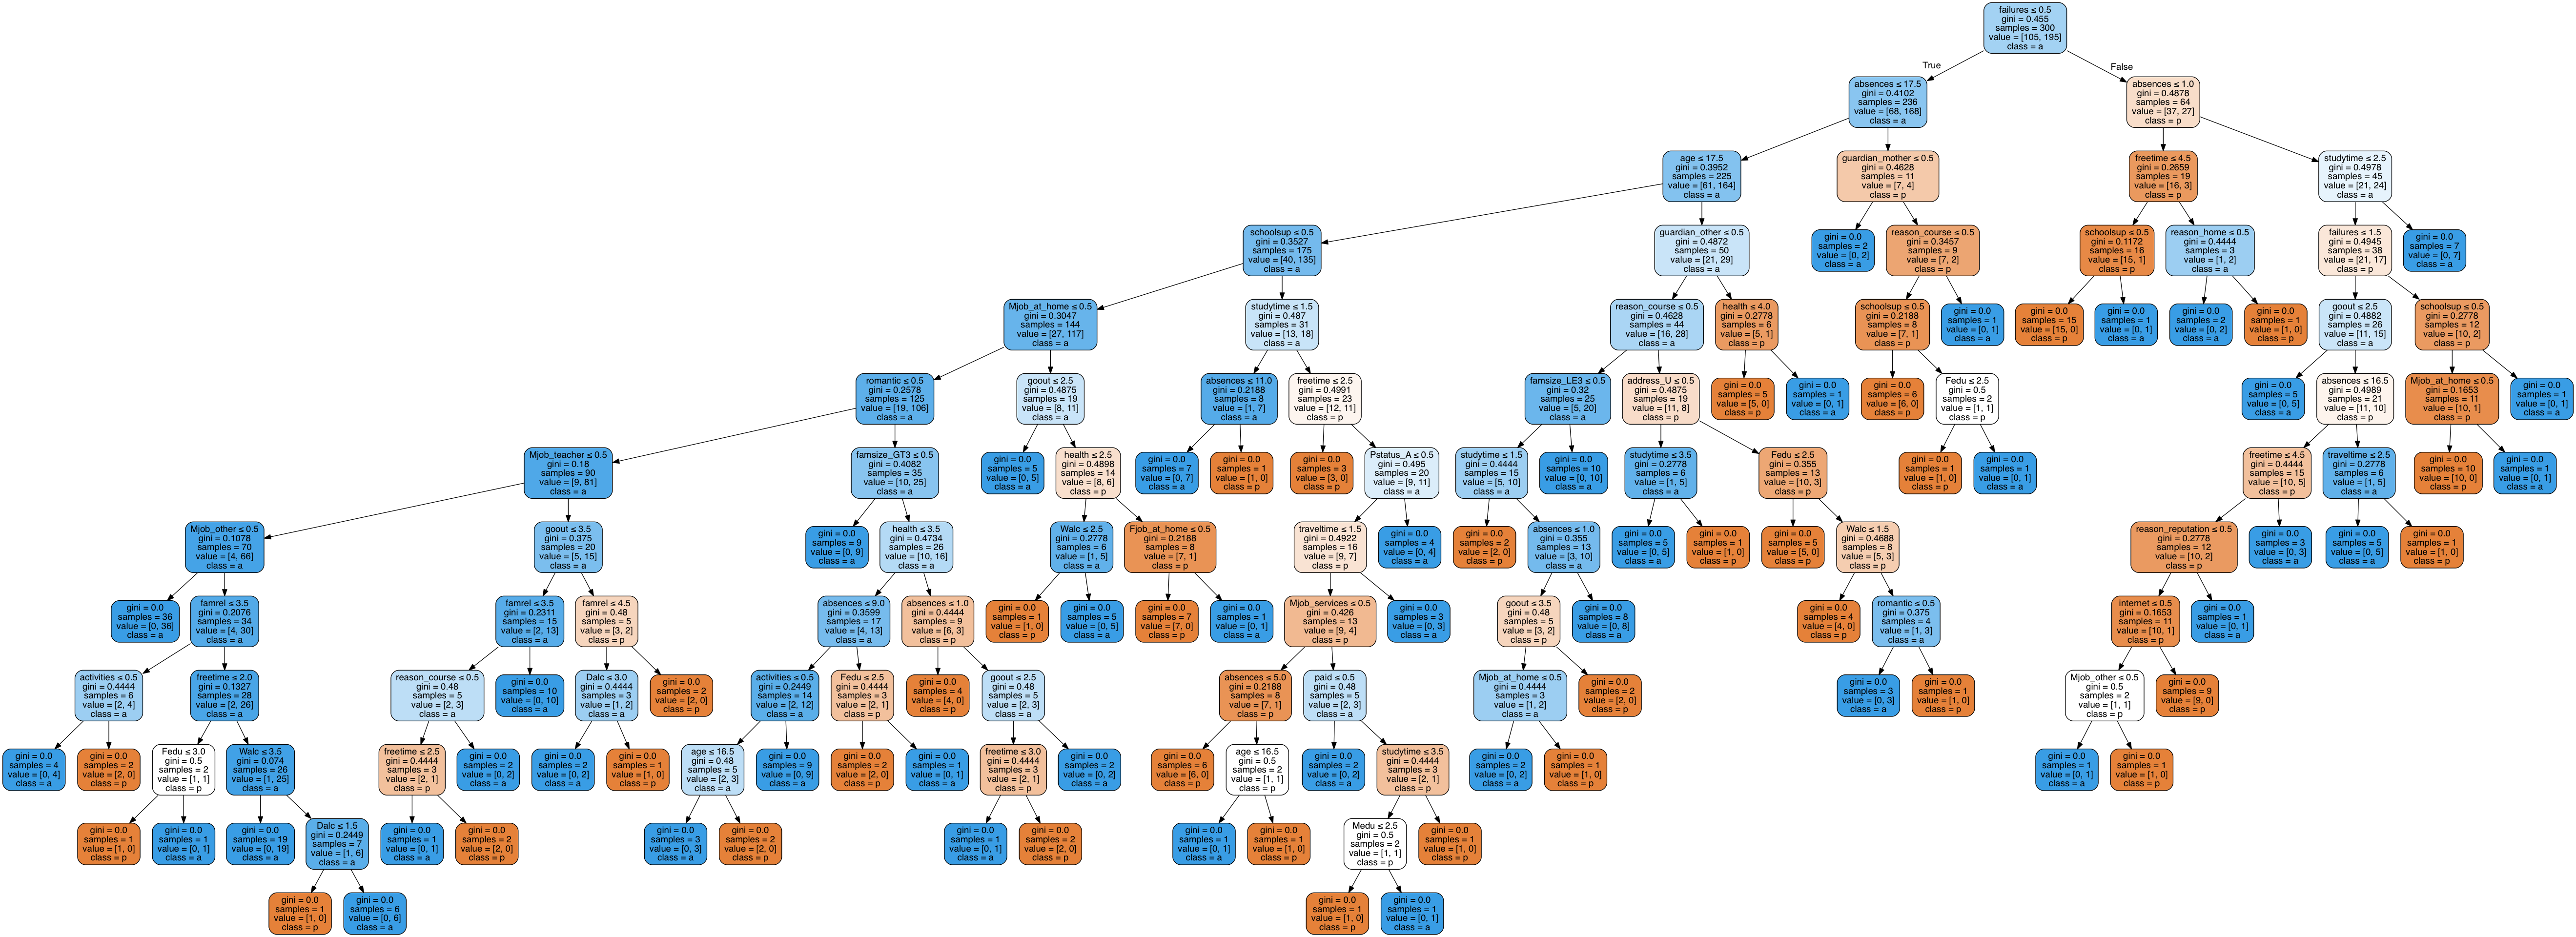
\includegraphics[width=1.0\textwidth]{tree} \\
\end{tabular}
\end{table}

\end{itemize}

\color{black}

\item In 1-3 paragraphs explain to the board of supervisors in layman's terms how the final model chosen is supposed to work (for example if you chose a decision tree or support vector machine, how does it learn to make a prediction).\\
\color{blue}
Logistic Regression learns from student data to find out relevant features so that it can predict who is likely to graduate and who may require early intervention.  It is a form of supervised machine learning model in that it is given labelled data and assigns weights to each feature in order to be able to predict using future data.\\
\\
In our case, the model is given data from students who did graduate and also who dropped out.  Each student is associated with 30 different feature set.  Different feature has different importance in terms of predicting students' probability to graduate. \\
\\
What Logistic Regression does is to adjust weights on each feature so that prediction error is minimized while training with students' data.  Once the training is done, we test it with independent students' data set aside for that purpose so that we do not overfit (i.e. the model is not adjusted too specific to the training data).\\
\\
Logistic Regression generates a probability for each student if they can graduate or not, which is then mapped to true/false value (i.e. false means he/she may require early intervention in order to graduate).\\
\\
It is recommended choice since it saves cost as it requires less memory and time resources, and yet it makes good prediction, and makes less mistakes even with small student data set.
\color{black}

\item Fine-tune the model. Use gridsearch with at least one important parameter tuned and with at least 3 settings. Use the entire training set for this.
\\
\color{blue}
Logistic Regression can overfit especially when training set size is smaller and there are many features.\\
\\
I've tried grid search to adjust the regularization to avoid such potential issue, and at the same time, improving the performance.\\
\\
With C=0.01, Logistic Regression performance improved (see the next section for details). \\

\color{black}

\item What is the model?s final F1 score?
\\
\color{blue}
The final F1 score is 0.8255 with all student data.
\\\\
For comparison with earlier results, here is the outcome with 100,200,300 training data.
The test performance improved with tuning.
\\\\
\begin{table}[H]
\centering
\begin{tabular}{| l | l | l | l |}
\hline
Traing set size           & 100 & 200 & 300 \\
\hline
Training time (secs)      & 0.001 & 0.002 & 0.002 \\
\hline
Prediction time (secs)    & 0.000 & 0.000 & 0.000 \\
\hline
F1 score for training set & 0.952 & 0.845 & 0.844 \\
\hline
F1 score for test set     & 0.761 & 0.710 & 0.759 \\
\hline      
\end{tabular}
\caption{Logistic Regression Without Tuning}
\end{table}

\begin{table}[H]
\centering
\begin{tabular}{| l | l | l | l |}
\hline
Traing set size           & 100 & 200 & 300 \\
\hline
Training time (secs)      & 0.001 & 0.002 & 0.002 \\
\hline
Prediction time (secs)    & 0.000 & 0.000 & 0.000 \\
\hline
F1 score for training set & 0.885 & 0.848 & 0.840 \\
\hline
F1 score for test set     & 0.786 & 0.737 & 0.780 \\
\hline      
\end{tabular}
\caption{Logistic Regression With Tuning}
\end{table}

\color{black}
\end{itemize}

\end{document}


